%-------------------------------------------------------------------------------
% Copyright (c) 2013-2016 University of Luxembourg.
% All rights reserved. This program and the accompanying materials
% are made available under the terms of the Eclipse Public License v1.0
% which accompanies this distribution, and is available at
% http://www.eclipse.org/legal/epl-v10.html
% 
% Contributors:
%     Alfredo Capozucca - initial writing
%      
%-------------------------------------------------------------------------------
%%%%%%%%%%%%%%%%%%%%%%%%%%%%%%%%%%%%%%%%%%%%%%%%%%
\PassOptionsToPackage{usenames,svgnames,table}{xcolor}
\documentclass[graybox,envcountchap,sectrefs]{./../lu.uni.lassy.excalibur.standard.report.libraries/styles/svmono}  
%%%%%%%%%%%%%%%%%%%%%%%%%%%%%%%%%%%%%%%%%%%%%%%%%%
%%% DO NOT CHANGE THE ORDER 
\usepackage{./../lu.uni.lassy.excalibur.standard.report.libraries/styles/style-messir-common}
\usepackage{./../lu.uni.lassy.excalibur.standard.report.libraries/styles/style-messir-report-post}
\usepackage{breakurl} 
\usepackage{float}
\usepackage{graphicx}
\usepackage{caption} 
%--------------------------------------------

% DOCUMENT BEGIN
%--------------------------------------------
\begin{document}

\newgeometry{textwidth=17cm,textheight=23.7cm}  
 
\definecolor{lightgray}{RGB}{201,201,201}
\definecolor{lightred}{RGB}{250,112,97}
\definecolor{lightgreen}{RGB}{179,250,140}

\definecolor{msrtextcl}{RGB}{0,0,0}
\definecolor{msrkeycl}{RGB}{127,0,85}
\definecolor{msrcmtcl}{RGB}{201,201,201}
\definecolor{keywordcolor}{RGB}{30,144,255}

\definecolor{aqua_blue}{RGB}{0,139,145}
\definecolor{dark_green}{RGB}{0,128,0}
\definecolor{dark_blue}{RGB}{45,45,138}

\definecolor{msrcolor01}{rgb}{0.96,0.59,0.48}
\definecolor{msrcolor02}{rgb}{1.00,0.97,0.60}
\definecolor{msrcolor03}{rgb}{0.51,0.79,0.61}
\definecolor{msrcolor04}{rgb}{0.43,0.81,0.96}
\definecolor{msrcolor05}{rgb}{0.52,0.58,0.79}
\definecolor{msrcolor06}{rgb}{0.96,0.61,0.76}
\definecolor{msrcolor07}{rgb}{0.98,0.68,0.51}
\definecolor{msrcolor08}{rgb}{0.77,0.88,0.61}
\definecolor{msrcolor09}{rgb}{0.49,0.66,0.85}
\definecolor{msrcolor10}{rgb}{0.96,0.60,0.62}
\definecolor{msrcolor11}{rgb}{0.64,0.83,0.61}
\definecolor{msrcolor12}{rgb}{0.63,0.53,0.75}
\definecolor{msrcolor13}{rgb}{0.99,0.78,0.54}
\definecolor{msrcolor14}{rgb}{0.53,0.51,0.74}
\definecolor{msrcolor15}{rgb}{0.48,0.80,0.79}
\definecolor{msrcolor16}{rgb}{0.74,0.55,0.75}
\definecolor{msrcolor17}{rgb}{0.90,0.79,0.08}
\definecolor{msrcolor18}{rgb}{1.00,1.00,0.00}
\definecolor{msrcolor19}{rgb}{1.00,0.00,0.50}

\definecolor{sepcolor000000}{rgb}{0, 0, 0}
\definecolor{sepcolor101010}{rgb}{0.10, 0.10, 0.10}
\definecolor{sepcolor202020}{rgb}{0.20, 0.20, 0.20}
\definecolor{sepcolor303030}{rgb}{0.30, 0.30, 0.30}
\definecolor{sepcolor404040}{rgb}{0.10, 0.10, 0.10}
\definecolor{sepcolor505050}{rgb}{0,1,.5}
\definecolor{sepcolor907908}{rgb}{0,1,.5}

\definecolor{sepregioncolor01}{rgb}{0.00,0.66,0.00}
\definecolor{sepregioncolor02}{rgb}{1.00,1.00,0.00}
\definecolor{sepregioncolor03}{rgb}{1.00,0.97,0.60}
\definecolor{sepregioncolor04}{rgb}{0.64,0.83,0.61}
\definecolor{sepregioncolor05}{rgb}{0.95,0.36,0.00}
\definecolor{sepregioncolor06}{rgb}{0.90,0.79,0.08}
\definecolor{sepregioncolor07}{rgb}{0.63,0.53,0.75}
\definecolor{sepregioncolor08}{rgb}{0.99,0.78,0.54}
\definecolor{sepregioncolor09}{rgb}{0.96,0.61,0.76}
\definecolor{sepregioncolor10}{rgb}{1.00,0.00,0.50}

\colorlet{msrcolorbrown}{red!40!black!80}


% Messir General
%----------------------------------------------------------

% quotePosition + quoteWidth + quotefillColor + quoteElement + quotedElement + allImageScale
\newcommand{\msrcallouted}[6]{
\scalebox{#1}{\parbox{\linewidth}{
  \begin{tikzpicture}
      \node [rectangle callout,callout relative pointer={#4},text width=#5,fill=#6,rounded corners] (tmpcall) at (0,0) {#3};
      \node at (tmpcall.pointer){#2};
  \end{tikzpicture}
}}
}

% Vresion wihtout scaling the quoted text
\pgfkeys{%
    /calloutquote/.cd,
    width/.code                   =  {\def\calloutquotewidth{#1}},
    position/.code                =  {\def\calloutquotepos{#1}}, 
    author/.code                  =  {\def\calloutquoteauthor{#1}},
    /calloutquote/.unknown/.code   =  {\let\searchname=\pgfkeyscurrentname
                                 \pgfkeysalso{\searchname/.try=#1,
    /tikz/\searchname/.retry=#1},\pgfkeysalso{\searchname/.try=#1,
                                  /pgf/\searchname/.retry=#1}}
                            }  

\newcommand\calloutquote[2][]{%
  \pgfqkeys{/calloutquote}{#1}
  \node [rectangle callout,callout relative pointer={\calloutquotepos},text width=\calloutquotewidth,/calloutquote/.cd,#1] (tmpcall) at (0,0) {#2};
  \node at (tmpcall.pointer){\calloutquoteauthor};    
}  
%----------------------------------------------------------
\newcommand{\msrTalkRD}[6]{
\freeblock{5}{#1}{#2}{
\begin{figure}
  \centering
  \includegraphics[width=#5]{images/various/descartes.pdf} 
\end{figure}
}
\freeblock{5}{#3}{#4}{
\scriptsize
\textit{#6}
}
}
\newcommand{\msrTalkGB}[6]{
\freeblock{5}{#1}{#2}{
\begin{figure}
  \centering
  \includegraphics[width=#5]{images/various/graham-bell.pdf} 
\end{figure}
}
\freeblock{5}{#3}{#4}{
\scriptsize
\textit{#6}
}
}
%----------------------------------------------------------

\newcommand{\msrQuestionSlide}[1]{
\begin{frame}[fragile]
\freeblock{5}{1}{4}{
\begin{figure}
  \centering
  \includegraphics[width=3cm]{images/various/3d-man-question-sit.pdf}
\end{figure}
}
\freeblock{10}{5}{3}{
\Large
\msrtxtclb{red}{\textit{#1}}
}
\end{frame}
}

%%%%%%%%%%%%%%%%%%%%%%%%%%%%%%%%%%%%%%%%%%%%%%%%%%%%%%%%%%
%%%%%%%%%%%%%%%%%%%%%%%%%%%%%%%%%%%%%%%%%%%%%%%%%%
%%% AUDIO
%%%%%%%%%%%%%%%%%%%%%%%%%%%%%%%%%%%%%%%%%%%%%%%%%%

\DeclareRobustCommand{\MyIncludeMedia}[5]{%
\addmediapath{#1}
\includemedia[
  flashvars={source=#2%
  &hideBar=true%
  &autoPlay=#3%
  },
  activate=pagevisible,
  noplaybutton,
  addresource=#2,
  transparent,
  passcontext
]{\includegraphics[width=.8cm]{#4}}{APlayer.swf}%
}

\DeclareRobustCommand{\slidesAudioModeChange}[1]
{\renewcommand{\slidesAudioMode}{#1}}

\DeclareRobustCommand{\slidesAudioHelp}{%
\IfSubStr{\slidesAudioMode}%
{remove}%
{}
{%
\pdfcomment[icon=Help,color=blue!10,open=false,subject={standard 14 fonts}]{Right clic on flag to have options !\\
Audio only available with Acrobat\ldots}%
}
}


\DeclareRobustCommand{\MyAudioButton}[3]{%
\IfSubStr{\slidesAudioMode}%
{remove}%
{}
{%
\IfSubStr{#1}{pause}{\def\MyAutoPlayMode{false}}{}%
\IfSubStr{#1}{\slidesAudioMode}{\def\MyAutoPlayMode{true}}{\def\MyAutoPlayMode{false}}%
\IfSubStr{#1}%
{fr}%
{\def\MyAudioIconPath{./../MessirSlides/images/various/flag-audio-FR.pdf}}{}%
\IfSubStr{#1}%
{en}%
{\def\MyAudioIconPath{./../MessirSlides/images/various/flag-audio-EN.pdf}}{}%
\IfSubStr{#1}%
{de}%
{\def\MyAudioIconPath{./../MessirSlides/images/various/flag-audio-DE.pdf}}{}%
\IfSubStr{#1}%
{lu}%
{\def\MyAudioIconPath{./../MessirSlides/images/various/flag-audio-LU.pdf}}{}%
\MyIncludeMedia{#2}{#3}{\MyAutoPlayMode}{\MyAudioIconPath}{#1}%
}
}
\makeatletter % we need to use kernel commands
\newcommand{\MyAudioBegin}{%
\begin{flushright}%
\setstretch{.3}
\@MyAudioOne%
}
\newcommand\@MyAudioOne{\@ifnextchar\stopaudio{\@MyAudioEnd}{\@MyAudioTwo}}

\newcommand\@MyAudioTwo[3]{%
\hspace*{-0.1cm}\@MyAudioThree{#1}{#2}{#3}%
\@MyAudioOne% restart the recursion
}
\newcommand\@MyAudioThree[3]{%
\MyAudioButton{#1}%
{#2}%
{#3}%
}
\newcommand\@MyAudioEnd[1]{% The argument is \stopaudio
\end{flushright}%
}
\makeatother

%%%%%%%%%%%%%%%%%%%%%%%%%%%%%%%%%%%%%%%%%%%%%%%%%%

\DeclareRobustCommand{\msrfigure}[4]{
\begin{figure}[htbp]
%\centering
\scalebox{#1}{
{\begin{minipage}[c]{\linewidth}
\centering
#2
\end{minipage}
}}
\ifthenelse{\equal{#4}{}}
             {}
             {\caption{#4}}
\label{#3}
\end{figure}
}

\newcommand{\semitransp}[2][30]{\color{fg!#1}#2}
\newcommand*{\msrtechfont}{\fontfamily{ptm}\selectfont}

\DeclareRobustCommand{\msruml}{{\msrtechfont UML}~}
\DeclareRobustCommand{\msrocl}{{\msrtechfont OCL}~}
\DeclareRobustCommand{\msromg}{{\msrtechfont OMG}~}
\DeclareRobustCommand{\msrxtext}{{\msrtechfont Xtext}~}
\DeclareRobustCommand{\msremf}{{\msrtechfont EMF}~}
\DeclareRobustCommand{\msrcm}{\msrcode{{Concept Model}}~}

\DeclareRobustCommand{\msrapache}{{\msrtechfont Apache}~}
\DeclareRobustCommand{\msratlassian}{{\msrtechfont Atlassian}~}
\DeclareRobustCommand{\msrbamboo}{{\msrtechfont Bamboo}~}
\DeclareRobustCommand{\msrconfluence}{{\msrtechfont Confluence}~}
\DeclareRobustCommand{\msreclemma}{{\msrtechfont EclEmma}~}
\DeclareRobustCommand{\msreclipse}{{\msrtechfont Eclipse}~}
\DeclareRobustCommand{\msrsql}{{\msrtechfont SQL}~}
\DeclareRobustCommand{\msrjava}{{\msrtechfont Java}~}
\DeclareRobustCommand{\msrjavafx}{{\msrtechfont JavaFx}~}
\DeclareRobustCommand{\msrjira}{{\msrtechfont JIRA}~}
\DeclareRobustCommand{\msrjunit}{{\msrtechfont JUnit}~}
\DeclareRobustCommand{\msrlatex}{{\msrtechfont Latex}~}
\DeclareRobustCommand{\msrmaven}{{\msrtechfont Maven}~}
\DeclareRobustCommand{\msrmysql}{{\msrtechfont MySQL}~}
\DeclareRobustCommand{\msrocl}{{\msrtechfont OCL}~}
\DeclareRobustCommand{\msrpdf}{{\msrtechfont PDF}~} 
\DeclareRobustCommand{\msrsirius}{{\msrtechfont Sirius}~} 
\DeclareRobustCommand{\msrsvn}{{\msrtechfont SubVersioN}~}
\DeclareRobustCommand{\msrswtbot}{{\msrtechfont SWTbot}~}
\DeclareRobustCommand{\msrxtext}{{\msrtechfont Xtext}~} 

 
\DeclareRobustCommand{\msrmessirmeth}{{\msrmessir}~methodology~}
\newcommand{\msrglsstyle}[1]{\emph{#1}}
\DeclareRobustCommand{\msrucname}[1]{\msrcode{\underline{#1}}}

% Verify macro since creates .toc errors
%\DeclareRobustCommand{\msrcode}[1]{{\normalfont\fontfamily{pcrr}\selectfont #1}}
%\DeclareRobustCommand{\msrcode}[1]{{\normalfont\fontfamily{cmvtt}\selectfont #1}}
\DeclareRobustCommand{\msrcode}[1]{{\protect\ \ttfamily \hyphenchar\font=`\- #1}}

% Messir Lexique
\DeclareRobustCommand{\msrbool}{\msrcode{{\emph Boolean}}~}
\DeclareRobustCommand{\msrint}{\msrcode{{\emph Integer}}~}
\DeclareRobustCommand{\msrreal}{\msrcode{{\emph Real}}~}
\DeclareRobustCommand{\msrstring}{\msrcode{{\emph String}}~}
\DeclareRobustCommand{\msrenum}{\msrcode{{\emph enumeration}}~}
\DeclareRobustCommand{\msrenums}{\msrcode{{\emph enumerations}}~}

% Messir Analysis
\DeclareRobustCommand{\msrsysop}{\emph{system operation}}
\DeclareRobustCommand{\msrsysops}{\emph{system operations}}
\DeclareRobustCommand{\msrsysintpro}{\emph{system interaction protocol}}
\DeclareRobustCommand{\msrbhvmd}{\emph{system operation}}

\newcommand{\msrt}[1]{\textuncl{#1}~}

\DeclareRobustCommand{\msrfont}[1]{\textuncl{#1}}
\DeclareRobustCommand{\msrfontb}[1]{\msrfont{\textbf{#1}}}
\DeclareRobustCommand{\msrfontcl}[1]{\msrfont{{\color{MediumPurple}#1}}}
\DeclareRobustCommand{\msrfontclb}[1]{{\msrfontcl{\textbf{#1}}}}

\DeclareRobustCommand{\msrcl}[1]{{\color{MediumPurple}#1}~}
\DeclareRobustCommand{\msrclb}[1]{{\msrcl{\textbf{#1}}}}

\DeclareRobustCommand{\msrmessir}{\msrfont{Messir}~}
\DeclareRobustCommand{\msrmessirb}{\msrfont{\textbf{Messir}}}
\DeclareRobustCommand{\msrmessircl}{{\color{MediumPurple}\msrmessir}}
\DeclareRobustCommand{\msrmessirclb}{{\color{MediumPurple}\msrmessirb}}

\DeclareRobustCommand{\msrexcalibur}{{\unclfamily Excalibur}~}
\DeclareRobustCommand{\msrexcaliburb}{\msrfont{\textbf{\msrexcalibur}}}
\DeclareRobustCommand{\msrexcaliburcl}{\msrfontcl{\msrexcalibur}}
\DeclareRobustCommand{\msrexcaliburclb}{\msrfontclb{\msrexcalibur}}

\DeclareRobustCommand{\msrmessim}{\msrfont{MesSim}}
\DeclareRobustCommand{\msrmessimb}{\msrfontb{MesSim}}
\DeclareRobustCommand{\msrmessimcl}{\msrfontcl{MesSim}}
\DeclareRobustCommand{\msrmessimclb}{\msrfontclb{MesSim}}

\DeclareRobustCommand{\msrmessam}{\msrfont{MesSam}}
\DeclareRobustCommand{\msrmessamb}{\msrfontb{MesSam}}
\DeclareRobustCommand{\msrmessamcl}{\msrfontcl{MesSam}}
\DeclareRobustCommand{\msrmessamclb}{\msrfontclb{MesSam}}

\DeclareRobustCommand{\msrmevop}{\msrfont{MevoP}~}
\DeclareRobustCommand{\msrmevopb}{\msrfontb{MevoP}~}
\DeclareRobustCommand{\msrmevopcl}{\msrfontcl{MevoP}~}
\DeclareRobustCommand{\msrmevopclb}{\msrfontclb{MevoP}~}

\DeclareRobustCommand{\msrmessep}{\msrfont{Messep}~}
\DeclareRobustCommand{\msrmessepb}{\msrfontb{Messep}~}
\DeclareRobustCommand{\msrmessepcl}{\msrfontcl{Messep}~}
\DeclareRobustCommand{\msrmessepclb}{\msrfontclb{Messep}~}

\DeclareRobustCommand{\msrmessee}{\msrfont{MesSEE}~}
\DeclareRobustCommand{\msrmesseeb}{\msrfontb{MesSEE}~}
\DeclareRobustCommand{\msrmesseecl}{\msrfontcl{MesSEE}~}
\DeclareRobustCommand{\msrmesseeclb}{\msrfontclb{MesSEE}~}

\DeclareRobustCommand{\msrprolog}{{\msrtechfont Prolog}}
\DeclareRobustCommand{\msrmessimb}{\textbf{\msrmessim}}
\DeclareRobustCommand{\msrprologcl}{\textcolor{red}{\msrprolog}}
\DeclareRobustCommand{\msrprologclb}{\textbf{\msrprologcl}}

\DeclareRobustCommand{\msrmcl}{{\footnotesize \msrfont{mcl}}}
\DeclareRobustCommand{\msrmclb}{\msrfontb{\msrmcl}}
\DeclareRobustCommand{\msrmclclb}{\msrfontcl{\msrmclb}}
\DeclareRobustCommand{\msrmclcl}{\msrfontcl{\msrmcl}}

\DeclareRobustCommand{\msrmcltt}{\protect\ \msrmessir Constraint Language~}
\DeclareRobustCommand{\msrmessimtt}{\protect\ \msrmessir Simulator~}
\DeclareRobustCommand{\msrmessamtt}{\protect\ \msrmessir Abstract Machine~}

\DeclareRobustCommand{\msrgeneric}{\textbf{\textit{{\color{MediumPurple}generic}}}~} 
\DeclareRobustCommand{\msrhelloworld}{\textbf{\textit{{\color{MediumPurple}HelloWorld}}}~}
\DeclareRobustCommand{\msricrash}{\textbf{\textit{{\color{MediumPurple}iCrash}}}~} 
\DeclareRobustCommand{\msricrashmini}{\textbf{\textit{{\color{MediumPurple}iCrashMini}}}~}  

\DeclareRobustCommand{\msrtxtcl}[2]{{\color{#1}#2}}
\DeclareRobustCommand{\msrtxtclb}[2]{\msrtxtcl{#1}{\textbf{#2}}}


%---------TABLES TEMPLATE--------------

%\rowcolors{2}{gray!20}{}

\newcounter{itemtable}


\newenvironment{usecase}{\begin{longtable}{|p{0.10\textwidth}
p{0.90\textwidth}|} \hline} {\hline \end{longtable}}


\newenvironment{usecaseinstance}{\begin{longtable}{|p{0.05\textwidth}
p{0.95\textwidth}|} \hline}
{\hline \end{longtable}}


\newenvironment{actortable}{
\begin{longtable}{|p{0.10\textwidth} p{0.90\textwidth}|}
\hline \hline}
{\hline \end{longtable}}


\newenvironment{datadictionary}{
\begin{longtable}{|p{0.15\textwidth} p{0.85\textwidth}|}
\hline \hline}
{\hline \end{longtable}}


\newenvironment{associationtypes}{
\begin{longtable}{|p{0.15\textwidth} p{0.85\textwidth}|}
\hline \hline}
{\hline \end{longtable}}


\newenvironment{operationmodel}{
\setcounter{itemtable}{0}
\begin{longtable}{|p{0.10\textwidth} p{0.90\textwidth}|}
\hline \hline}
{\hline \end{longtable}}


\newenvironment{teststepmodel}{
\setcounter{itemtable}{0}
\begin{longtable}{|p{0.10\textwidth}|p{0.90\textwidth}|}
\hline}
{\hline \end{longtable}}


\newcommand*{\myfont}{\fontfamily{phv}\selectfont}


\newcommand\addheading[1]{
\hline
%\multicolumn{2}{|l|}{\cellcolor[gray]{0.9} \textbf{#1}} \\
\multicolumn{2}{|l|}{\textbf{\scshape #1}} \\
\hline \hline
\endfirsthead

\multicolumn{2}{@{}l}{\myfont{\bfseries\itshape{\ldots #1 table
continuation}}}\\
%\hline \hline
%\multicolumn{2}{|l|}{\cellcolor[gray]{0.9} \textbf{#1}}\\
%\hline \hline
\endhead % all the lines above this will be repeated on every page

%\hline \hline
\multicolumn{2}{r@{}}{\myfont{\bfseries\itshape{continues in next page
\ldots}}}\\
\endfoot

\hline
\endlastfoot}

%\multicolumn{2}{|l|}{\cellcolor[gray]{0.8}
\newcommand\addrowheading[1]{
\hline \hline
\multicolumn{2}{|l|}{
  \setcounter{itemtable}{0}
  \textbf{\itshape #1}}\\
\hline \hline
}


\newcommand\addsinglerow[1]{
\multicolumn{2}{|l|}{\begin{minipage}[t][][t]{1.0\textwidth}
#1 \end{minipage}} \\
%\hline
}


\newcommand\addsingletwocolumnrow[2]{
{\itshape #1} & #2 \\
%\hline
}


\newcommand\adddoublerow[2]{
\hline \hline
\multicolumn{2}{|l|}{\begin{minipage}[t][][t]{1.0\textwidth}
\textbf{\itshape #1} \end{minipage}} \\
\multicolumn{2}{|l|}{\begin{minipage}[t][][t]{1.0\textwidth}
#2 \end{minipage}} \\
\hline
}


\newcommand\adddoubletwocolumnrow[3]{
#1 & \textbf{#2} \\
& #3 \\
%\hline
}


\newcommand\addnumberedsinglerow[2]{
\stepcounter{itemtable}
\text{#1 \theitemtable} & #2 \\
%\hline
}


\newcommand\addnumbereddoublerow[3]{
\stepcounter{itemtable}
\text{#1 \theitemtable} & \textbf{#2} \\
       & #3 \\
%\hline
}



\newcommand\addalphanumberedsinglerow[2]{
\stepcounter{itemtable}
\text{#1 \alph{itemtable}} & #2 \\
%\hline
}


\newcommand\addalphanumbereddoublerow[3]{
\stepcounter{itemtable}
\text{#1 \alph{itemtable}} & \textbf{#2} \\
       & #3 \\
%\hline
}

%%%%%%%%%%%%%%%%%%%%%%%%%%%%%%%%%%%%%%%%%%%%%%%%%%%%%%%%%%%%%%%%%%%%%%%%%%%%
%%%%%%%%%%%%%%%%%%%%%%%%%%%%%%%%%%%%%%%%%%%%%%%%%%%%%%%%%%%%%%%%%%%%%%%%%%%%

\lstdefinelanguage{MessirProlog}{
morekeywords=[1]{msrNav,msrop,:-},
morekeywords=[2]{msrVar},
morekeywords=[3]{msrTrue,msrFalse,true,false,msrIsNew,msrIsKilled,msrForAll,msrExists,msrSelect,msrReject,msrClose,msrAny,msrIsEmpty,msrSize,msmAtPre,msmAtPost,msrColEq,msrColSubtract,msrCount,msrExcludes,msrExcludesAll,msrIncludes,msrIncludesAll,msrSum,msrProd,msrIncluding,msrExcluding,msrIntersection,msrUnion,msrAsSet,msrOne},
morekeywords=[3]{rnSystem,rnActor,rnSystem,rnInterfaceIN,rnInterfaceOUT,ptBoolean,ptReal,ptString,ptInteger,preProtocol,preFunctional,postProtocol,postFunctional,init},
morekeywords=[4]{Self},
sensitive=true,
morestring=[b]{"},
comment=[s]{/*}{*/},
morecomment=[l]//
}[keywords,comments,strings]%
 
\lstdefinestyle{MessirPrologStyle} { 
language=MessirProlog,
extendedchars=true,
basicstyle=\ttfamily,
%keywordstyle=\color{blue}\bfseries,
keywordstyle=[1]\color{blue}\bfseries,
keywordstyle=[2]\color{red},
keywordstyle=[3]\color{msrcolor12}\bfseries,
keywordstyle=[4]\color{msrcolor09}\bfseries,
stringstyle=\color{msrtextcl},
commentstyle=\color{msrcmtcl},
breakatwhitespace=false,
tabsize=1,
literate={\ \ }{{\ }}1,
breaklines=true,
emptylines=1,
numbers=left,
numberstyle=\tiny\color{blue}, 
firstnumber=auto,
stepnumber=1,
numbersep=0pt, 
showspaces=false,
showlines=false,
numberfirstline=true,
showstringspaces=false
showtabs=false,
includerangemarker=true
}



\lstdefinestyle{MessirStyle} { 
language=Messir,
extendedchars=true,
basicstyle=\ttfamily,
keywordstyle=\color{msrkeycl}\bfseries,
stringstyle=\color{msrtextcl},
commentstyle=\color{msrcmtcl},
breakatwhitespace=false,
tabsize=1,
literate={\ \ }{{\ }}1,
breaklines=true,
emptylines=1,
numbers=left,
numberstyle=\tiny\bfseries\color{blue}, 
firstnumber=auto,
stepnumber=1,
numbersep=2pt, 
showspaces=false,
showlines=false,
numberfirstline=true,
showstringspaces=false
showtabs=false,
includerangemarker=true
}

\lstdefinelanguage{Messir}{
keywords={package,import,Concept,Model,Primary,Types,Secondary,state,class,
role,cardinality,extends,attribute,external,operation,primitive,
datatype,enum,constants,association,aggregation,composition,Environment,
actor,role,input,interface,output,Operation,external,link,preF,preP,postF,
postP,ocl,Test,test,case,order,step,prolog},
morekeywords=[1]{self,let,in,true,false,result},
morekeywords=[2]{name,attributes,associatoinEnds,operations,%
      supertypes,allSupertypes,allInstances,oclIsKindOf,oclIsTypeOf,%
      oclAsType,oclInState,oclIsNew,evaluationType,abs,floor,round,max,%
      min,div,mod,size,concat,toUpper,toLower,substring,includes,%
      excludes,count,includesAll,exludesAll,isEmpty,notEmpty,sum,%
      exists,forAll,isUnique,sortedBy,iterate,union,intersection,%
      including,excluding,symmetricDifference,select,reject,collect,%
      asSequence,asBag,asSequence,asSet,append,prepend,subSequence,at,%
      first,last,true,false,isQuery,context,pre,inv,post},
    morekeywords=[3]{and,equiv,exit,impl,not,or},%
    morekeywords=[4]{Boolean,Integer,Real,String,Set,Sequence,Bag,%
       OclType,OclAny,OclExpression,Enumeration,Collection},%
    morekeywords=[5]{Use,use,system,Case,Model,related,instance,primary,secondary,oracle,value,constraint,message,parameter,value,truth,protocol,functional,variables,values,results,subfunction,usergoal,summary,executes,sends,to,reuse,received,from,ordering,if,then,else,endif,self,^},
    morekeywords=[6]{executed,instanceof,returned,steps,active,passive,proactive,constraints,multiple},
    morekeywords=[7]{@Actor,@actorDeclaration,@actorSpecification,@additionalInformation,@attribute,@caption,@colOperation,@constraint,@description,@endActorsDeclaration,@endActorsSpecification,@endAttributes,@endColOperations,@endConstraints,@endInputEvents,@endInputParametersDeclaration,@endInputParametersSpecification,@endInstanceOracleOutputParameters,@endInstanceTestReceivedMessages,@endOperations,@endOracleConstraints,@endOracleOutputParametersSpecification,@endOracleReceivedMessagesSpecification,@endOracleValues,@endOracleVariables,@endOutputEvents,@endOutputParametersDeclaration,@endOutputParametersSpecification,@endParameters,@endPostConditions,@endPostF,@endPostP,@endPreConditions,@endPreF,@endPreP,@endProtocolConditions,@endRemarks,@endStepOrderingConstraints,@endVariables,@endVariableValues,@example,@inputEvent,@inputParameterDeclaration,@inputParameterSpecification,@Instance,@instanceOracleOutputParameter,@instanceTestReceivedMessage,@level,@model,@number,@Operation,@oracleConstraint,@oracleOutputParameterSpecification,@oracleReceivedMessageSpecification,@oracleSpecification,@oracleTruthValue,@oracleValue,@oracleVariable,@orientation,@outputEvent,@parameter,@postCondition,@postF,@postP,@preCondition,@preF,@preP,@Primary,@protocolCondition,@remark,@return,@scale,@Secondary,@stepOrderingConstraint,@sublevel,@Test,@testResultPostFunctional,@testResultPreFunctional,@testResultPreProcotol,@testSentMessage,@testSentMessageValue,@Use,@variable,@variableValue,@view,@pre,@post},
    morekeywords=[8]{@@Use,@@Instance,@@Primary,@@Secondary,@@Actor,@@Operation,@@Test,@@Instance,@@view,@operation},
sensitive=true,
morestring=[b]{"},
comment=[s]{/*}{*/},
morecomment=[l]//
%alsodigit={.}
}[keywords,comments,strings]%
%%%%%%%%%%%%%%%%%%%%%%%%%%%%%%%%%%%%%%%%%%%%%%%%%%%%%%%%%%%%%%%%%%%%%%%%%%%%
%%%%%%%%%%%%%%%%%%%%%%%%%%%%%%%%%%%%%%%%%%%%%%%%%%%%%%%%%%%%%%%%%%%%%%%%%%%%

%%%%%%%%%%%%%%%%%%%%%%%%%%%%%%%%%%%%%%%%%%%%%%%%%%%%%%%%%%%%%%%%%
%%%%%%%%%%%%%%      150506    %%%%%%%%%%%%%%%%%%%%%%%%%%%%%%%%%%%
%%%%%%%%%%%%%%%%%%%%%%%%%%%%%%%%%%%%%%%%%%%%%%%%%%%%%%%%%%%%%%%%%

\DeclareRobustCommand{\msrsee}{software engineering environment~}

\newcommand\freeblock[4]{%
\begin{textblock}{#1}(#2,#3)
\begin{minipage}{\textwidth}
\setlength{\parindent}{0pt}%
\setlength{\parskip}{0.1cm}%
#4
\end{minipage}
\end{textblock}
}

\newcommand\addheadingPS[4]{
\hline
\multicolumn{2}{|l|}{\textbf{\scshape Process Step}} \\
\hline
\multicolumn{2}{|l|}{Phase: \msrclb{#1} - Iteration: \msrclb{#2} - Step: \msrclb{#3}}\\
\hline
\multicolumn{2}{|l|}{Name: \msrclb{#4}}\\
\hline \hline
\endfirsthead 

\multicolumn{2}{@{}l}{\myfont{\bfseries\itshape{\ldots #1 table
continuation}}}\\
\endhead % all the lines above this will be repeated on every page

\multicolumn{2}{r@{}}{\myfont{\bfseries\itshape{continues in next page
\ldots}}}\\
\endfoot

\hline
\endlastfoot}

\newenvironment{processsteptable}{
\setcounter{itemtable}{0}
\begin{longtable}{|p{0.10\textwidth}|p{0.90\textwidth}|}
\hline}
{\hline \end{longtable}
}

%%%%%%%%%%%%%%%%%%%%%%%%%%%%%%%%%%%%%%%%%%%%%%%%%%
\newcommand{\mybox}[2]{\par\noindent\colorbox{#1}
{\parbox{\dimexpr\textwidth-2\fboxsep\relax}{#2}}}

\urlstyle{tt}
\newcommand{\msrurl}[3]{\href{#2}{\color{#1}{#3}}}%

%for time line tables
\newcommand\ytl[5]{
\parbox[b]{10em}{\hfill{\color{#2}\bfseries\sffamily #3}~$\cdots\cdots$~}\makebox[0pt][c]{$\bullet$}\vrule\quad \parbox[c]{\textwidth}{\vspace{#1pt}\color{#4}\raggedright\sffamily #5\\[7pt]}\\[-3pt]}

% For setting item spacing
% ex: {\setlistspacing{2}{2ex} \begin{frame} \ldots \end{frame}}
\makeatletter
\newcommand{\setlistspacing}[2]{\def\@ld{#1}\expandafter\def\csname
@list\romannumeral\@ld \endcsname{\leftmargin\csname
leftmargin\romannumeral\@ld \endcsname
              \topsep    #2
              \parsep    0\p@   \@plus\p@
              \itemsep   #2}}
\makeatother




\newglossaryentry{Concept Model}
{name={Concept Model},
description={the Model that describes the different types required to specify
the software system.}, 
plural={Concept Models},
symbol={\msrglsstyle{Concept Model}}
}

\newglossaryentry{Environment Model} 
{name={Environment Model},
description={the Model that describes the different actors supposed to interact
with the software system.}, 
plural={Environment Models},
symbol={\msrglsstyle{Environment Model}}
}



\newglossaryentry{MVC} 
{name={Model-View-Controller},
description={the pattern followed to design the Graphical User Interfaces
of the software system.}, 
plural={Model-View-Controllers}, 
symbol={\msrglsstyle{Model-View-Controller}}
}


\newglossaryentry{Design Model} 
{name={Design Model},
description={The Design Class Model is composed of the contents of all design classes, i.e.
their (value) attributes and methods, all the navigable associations between
design classes, and the inheritance structure. The Design Class Model has to be
modelled as a UML Class Diagram.}, 
plural={Design Models}, 
symbol={\msrglsstyle{Design Model}}
}


\newglossaryentry{Interaction Model} 
{name={Interaction Model},
description={The Interaction Model shows how objects are expected to interact at run-time to
support the \emph{system operations} specified in the \emph{Operation Model}
made during the Analysis Phase. There must exist an \emph{Interaction Model} for
each system operation specified in the \emph{Operation Model}. An Interaction Model has to be
modelled as a UML Sequence Diagram.}, 
plural={Interaction Models}, 
symbol={\msrglsstyle{Interaction Model}}
}

\newglossaryentry{Deployment View} 
{name={Deployment View},
description={The physical view depicts the system from a system engineer's
point-of-view. It is concerned with the topology of software components on the
physical layer, as well as the physical connections between these components.
For example, how many nodes are used and what is deployed on what node. A
Deployment View is modelled as a UML Deployment Diagram.}, 
plural={Deployment Views}, 
symbol={\msrglsstyle{Deployment View}}
}


\newglossaryentry{Implementation View} 
{name={Implementation View},
description={This view describes the software system components. It focuses on
software modules and subsystems. It describes the hierarchies or layers for
components. This view is modelled as a UML Component Diagram.},
plural={Implementation Views}, 
symbol={\msrglsstyle{Implementation View}}
}


\newglossaryentry{UI Processing View} 
{name={UI Processing View},
description={A Processing view is aimed at explaining the required
object interactions that allow a system operation to be called. A
UI Processing View is modelled as a UML Sequence Diagram.},
plural={UI Processing Views},
symbol={\msrglsstyle{UI Processing View}} }


\newglossaryentry{iCrash.FX} 
{name={iCrash Distributed Desktop development},
description={Implementation of the \msricrash case study made in \emph{Java} and
capable of ensuring a distributed execution.},
symbol={\msrglsstyle{iCrash.FX}} }





%  General Messir Glossary
\newglossaryentry{real number}
{name={Real number},
description={name of the set of real numbers.},
plural={reals},
symbol={\ensuremath{\mathbb{R}}}
}

\newglossaryentry{system operation}
{name={System Operation},
description={a functionality of the system that can be triggered by a message
sent by an actor belonging to the environment.}, plural={system operations},
symbol={\msrglsstyle{system operation}}
}


\newglossaryentry{societics}
{name={Societics},
description={Represents the fields of hardware/software
systems used for the society extension.}, 
symbol={\msrglsstyle{societics}}
}

\newglossaryentry{direct actor}
{name={Direct Actor},
description={an actor that interacts directly with the system. It thus belongs
to the environment.},
plural={direct actors},
symbol={\msrglsstyle{direct actor}}
}

\newglossaryentry{indirect actor}
{name={Indirect Actor},
description={an actor that interacts indirectly with the system through a direct
actor.  It thus belongs the domain but not to the environment.}, 
plural={indirect actors},
symbol={\msrglsstyle{indirect actor}}
}

\newglossaryentry{abstract actor}
{name={Abstract Actor},
description={an actor that does not exist in real life.},
plural={abstract actors},
symbol={\msrglsstyle{abstract actor}}
}

\newglossaryentry{socext}
{name={Society extension},
description={The society obtained by grouping people using natural means
extended with artificial means.},
symbol={\msrglsstyle{societics}}
}

\newglossaryentry{usecase}
{name={Use case},
description={A use case describes a sequence of actions that provide something
of measurable value to an actor. and is drawn as a horizontal ellipse.},
plural={Use cases}, 
symbol={\msrglsstyle{Use case}} 
}

\newglossaryentry{actor}
{name={Actor},
description={An actor is a person, organization, or external system that plays a
role in one or more interactions with the system.},
plural={actors},
symbol={\msrglsstyle{actor}}
}

\newglossaryentry{socialware}
{name={Societics},
description={Represents the fields of hardware/software
systems used for the society extension.},
symbol={\msrglsstyle{Societics}}
}

% \newglossaryentry{}
% {name={\msrglsstyle{}},
% description={},
% symbol={\msrglsstyle{actor}} }


%TITLE
%******************************************
\title{
\begin{tabular}{|>{\centering\arraybackslash\hspace{0pt}}p{16cm}|}
\hline
	\textbf{iCrashVariantG06:}\\
	\textbf{Crisis Management System}\\
	\textbf{Design Document}\\
	\textbf{ - v 0.2 - }\\
\hline 
\end{tabular}
\vspace{2cm}}
 
%******************************************
\author{
\begin{tabular}{l}
		Maria Kocherga\\
		Kuzma Leshakov\\
		Nikita Kurylenko\\
		\\Innopolis University\\
\end{tabular}}

\date{\today~-~\currenttime}
%****************************************************


\maketitle
\newpage

%TOC
\setcounter{tocdepth}{2}
\addtocounter{secnumdepth}{2}
\tableofcontents
\newpage

%TOF
\listoffigures
\newpage

%TOL
\lstlistoflistings
\newpage

%DOCUMENT STRUCTURE

% Introduction
\chapter{Introduction}
\label{chap:introduction}


\section{Scope}
Introduction scope goes right here. An example of using glossay might be. Zzzz 


This document \gls{KuzmaTerm}  provides \ldots
%Example: This document provides minimum acceptable information for knowing how
% to use the software system \mysystemname.


This document does not \ldots 
 
This document is not \ldots
%Example: This document is not intended to provide information about how to
% connect, deploy, configure, or use any external device or
% third-party software system that is rqeuired for the correct funcitoning of
% \mysystemname.

 
This document may be used with \ldots
%This document may be used with other documents provided by third-party
% companies to have an overall view and correct understanding of the environment
% and procedures where the software system \mysystemname is aimed to be deployed
% and run.




\section{Purpose}
In this section you explain the purpose (i.e. aim, objectives) of the user's
manual. In the following some examples of opening statements to be used in this
section. W  

The purpose of this document is \ldots

This document defines \ldots

This document is meant to \ldots



\section{Intended audience}
Description of the categories of persons targeted by this document together with the description of how they are expected to exploit the content of the document.


\section{\mysystemname}
Here 
  
   

\subsection{Actors \& Functionalities}
Overview of all the \textbf{\emph{\glspl{actor}}} interacting with the software
being them either humans (called end-users in the standard
\cite{IEEE-2001-userdocumentation}) or not. For each actor, describe the main
software functions that are offered to him. Structure of this sub-section MUST
be by actor/functionalities.


\subsection{Operating environment}
Brief overview of the infrastructure on which the software is deployed and used.

\section{Document structure}  
Information on how this document is organised and it is expected to be
used. Recommendations on which members of the audience
should consult which sections of the document, and explanations about the used
notation (i.e. description of formats and conventions) must also be provided.






\newpage

% Analysis Models 
\chapter{Analysis Models}
\label{chap:AM}

%This chapter provides a general overview of the main concepts gathered during
%the analysis phase, in particular those concerning the software system types
%(i.e. classes, datatypes, and enumerations), as well as the actors that
% interact with the software system through their interfaces. Figures included in the
%Messir Requirement Document that correspond to the  the \glspl{Concept Model}
% and the \glspl{Environment Model} could be also included in this chapter, as a means of synthesizing what
%are the requirements to which the design is supposed to sketch a solution.


\section{Flow-orineted model}
This model provides an indication of how data objects are transformed by a set
of processing functions.

\begin{figure}[h]
	\centering	
	\captionsetup{justification=centering}
	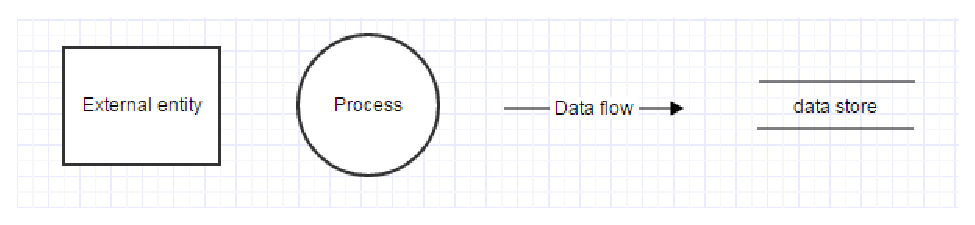
\includegraphics[width=0.5\textwidth]{./images/flow_notation.eps}
	\caption{Data Flow notation}
\end{figure}


\begin{figure}[h]
	\centering
	\captionsetup{justification=centering}
	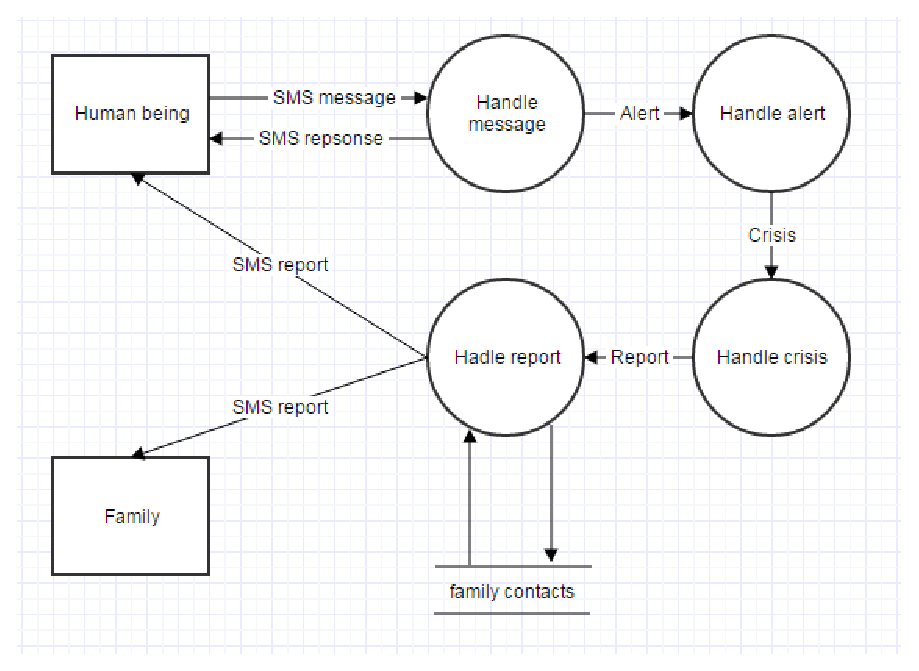
\includegraphics[width=0.5\textwidth]{./images/data_flow_diagram.eps}
	\caption{Data Flow diagram}
\end{figure} 

\section{Csenario-based model}
This model represents the system from the user's point of view.

\subsection{Use Cases}

\subsubsection{summary-suDeployAndRun}

The goal is to install the iCrash system on its infrastructure and to exploit its capacities related to the
secure administration and eficient handling of car crash situations depending on
alerts received.


\begin{figure}[h]
	\centering	
	\captionsetup{justification=centering}
	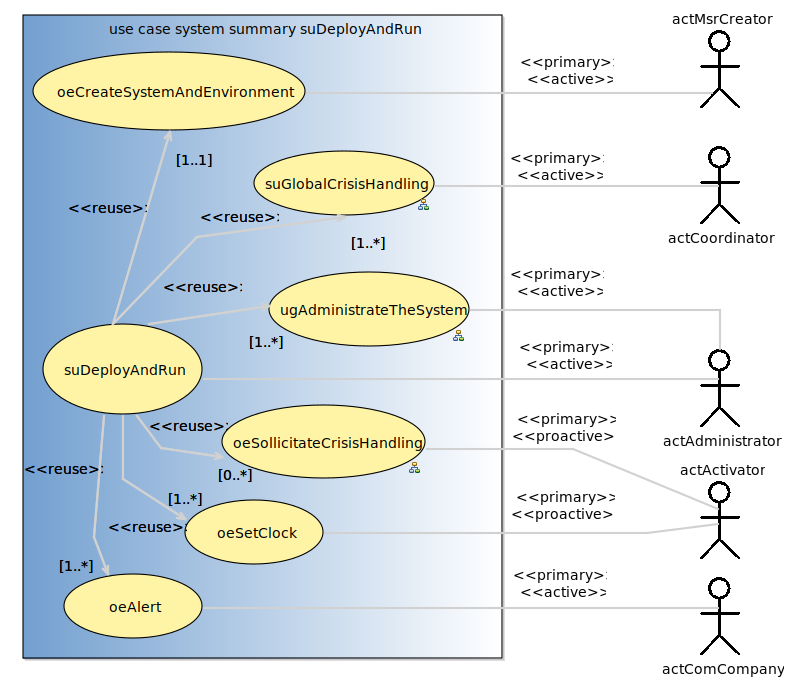
\includegraphics[width=0.5\textwidth]{./images/uc-suDeployAndRun.eps}
	\caption{Use case diagram for the suDeployAndRun summary use case}
\end{figure}


\section{Concept Model}
 

\begin{figure}[H]
	\centering
	\captionsetup{justification=centering}
	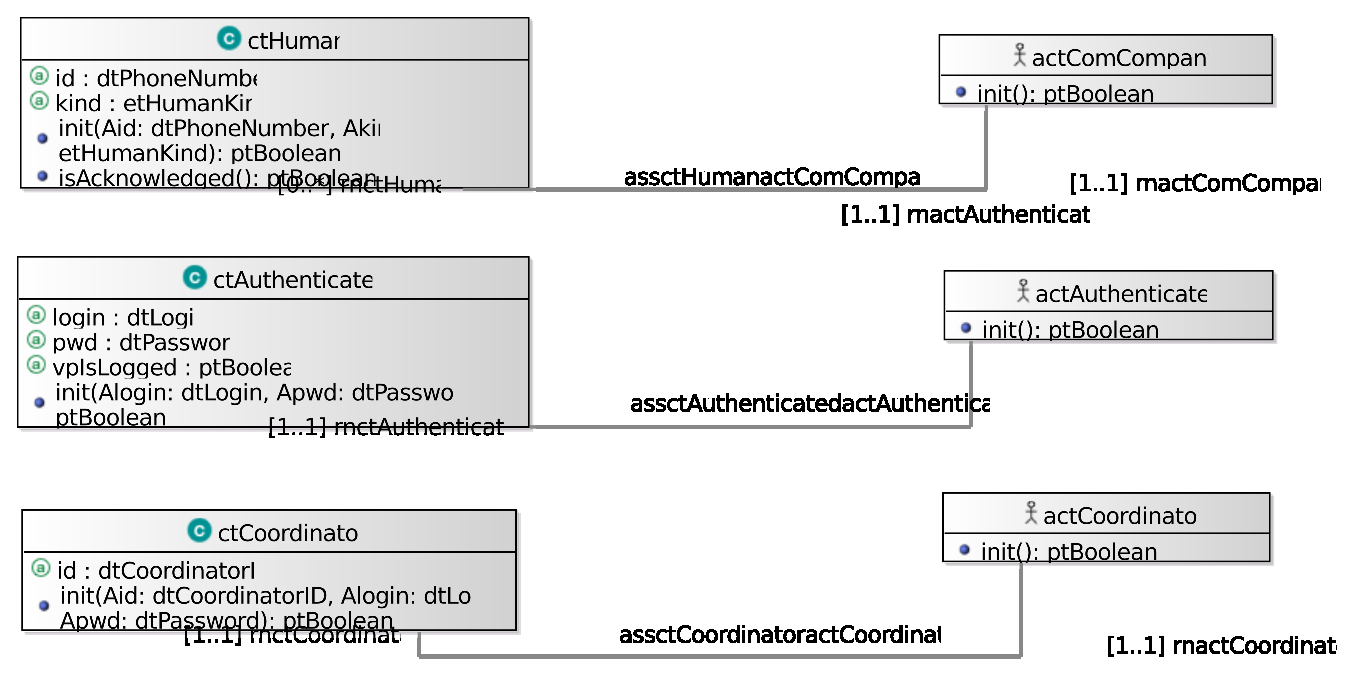
\includegraphics[width=0.5\textwidth]{./images/cm-pt-ct-gv-01.eps}
	\caption{Concept Model - PrimaryTypes-Classes local view 01. Local view of all the primary types
class types }
\end{figure} 

\begin{figure}[H]
	\centering
	\captionsetup{justification=centering}
	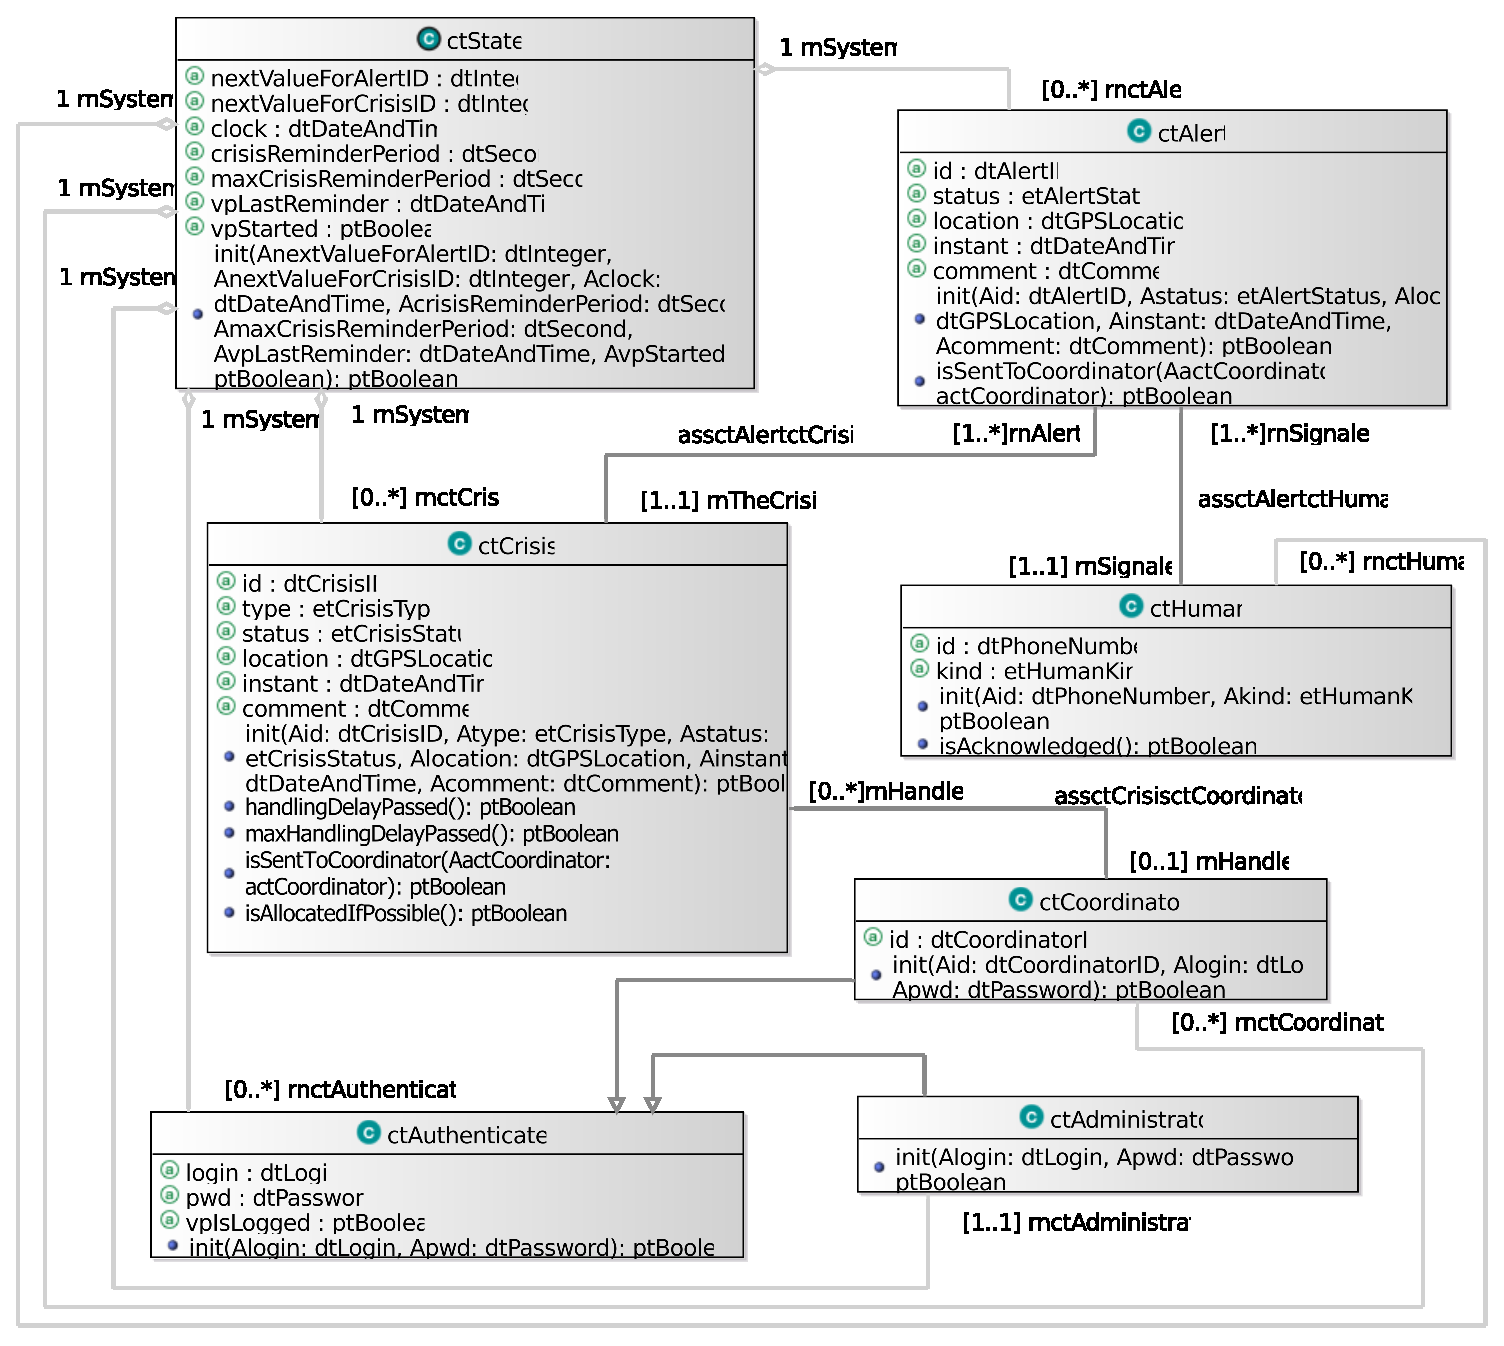
\includegraphics[width=0.5\textwidth]{./images/cm-pt-ct-lv-01.eps}
	\caption{Concept Model - PrimaryTypes-Classes local view 02. local view of the ctState primary
type.}
\end{figure} 

\begin{figure}[H]
	\centering
	\captionsetup{justification=centering}
	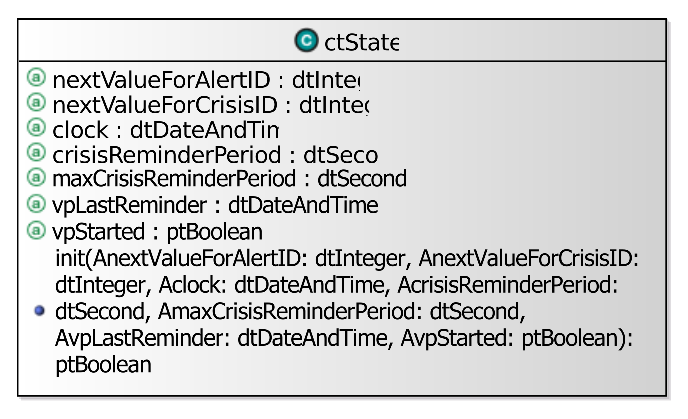
\includegraphics[width=0.5\textwidth]{./images/cm-pt-ct-lv-02-parta-ctState.eps}
	\caption{Concept Model - PrimaryTypes-Classes local view 03. local view of the ctAlert primary
type.}
\end{figure} 

\begin{figure}[H]
	\centering
	\captionsetup{justification=centering}
	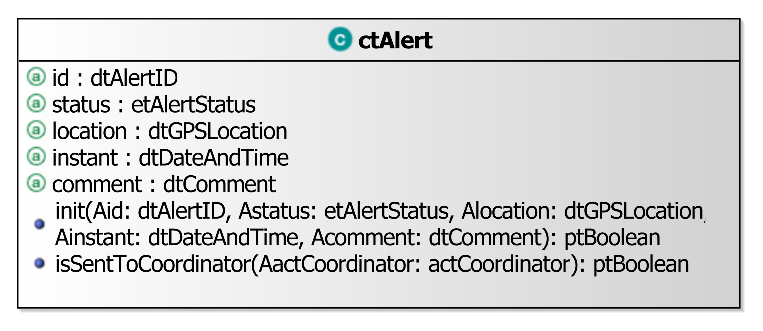
\includegraphics[width=0.5\textwidth]{./images/cm-pt-ct-lv-03-partb-ctAlert.eps}
	\caption{Concept Model - PrimaryTypes-Classes local view 04. local view of the ctCrisis primary
type.}
\end{figure} 

\begin{figure}[H]
	\centering
	\captionsetup{justification=centering}
	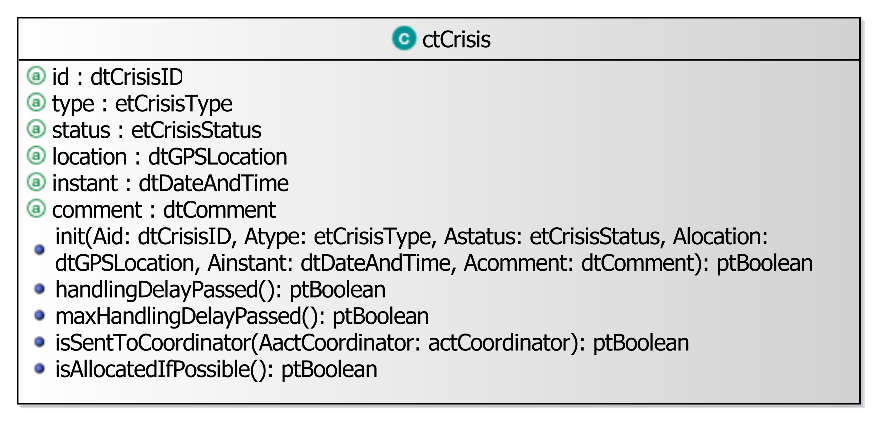
\includegraphics[width=0.5\textwidth]{./images/cm-pt-ct-lv-04-partc-ctCrisis.eps}
	\caption{Concept Model - PrimaryTypes-Classes global view 01. Primary types class types global
view - cm-pt-ct-gv-01 .}
\end{figure} 

\begin{figure}[H]
	\centering
	\captionsetup{justification=centering}
	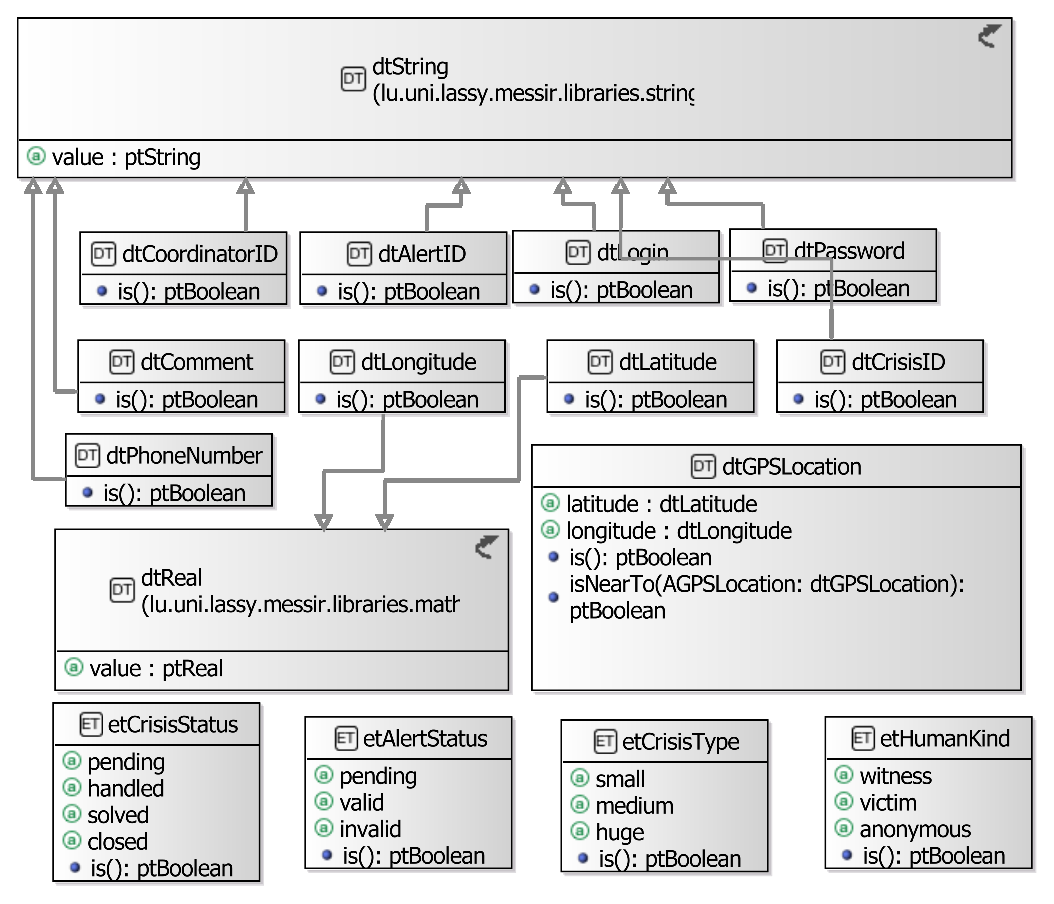
\includegraphics[width=0.5\textwidth]{./images/cm-pt-dt-gv-01.eps}
	\caption{Concept Model - PrimaryTypes-Datatypes local view 06.}
\end{figure} 

\begin{figure}[H]
	\centering
	\captionsetup{justification=centering}
	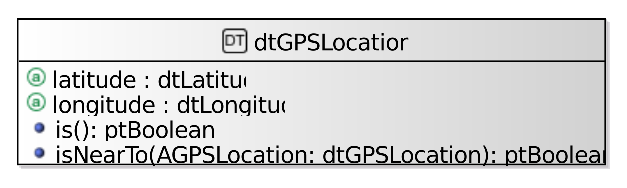
\includegraphics[width=0.5\textwidth]{./images/cm-pt-dt-lv-02-dtGPSLocation.eps}
	\caption{Concept Model - PrimaryTypes-Datatypes global view 01. global view of primary types
datatype types - cm-pt-dt-gv-01 .}
\end{figure} 

\begin{figure}[H]
	\centering
	\captionsetup{justification=centering}
	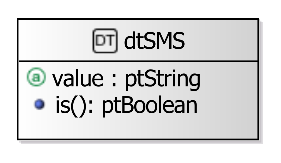
\includegraphics[width=0.5\textwidth]{./images/cm-st-dt-lv-01.eps}
	\caption{Concept Model - SecondaryTypes-Datatypes local view 01. Local view of the secondary
types datatype types.}
\end{figure} 
   

\section{Environment Model}

\begin{figure}[h]
\begin{center}
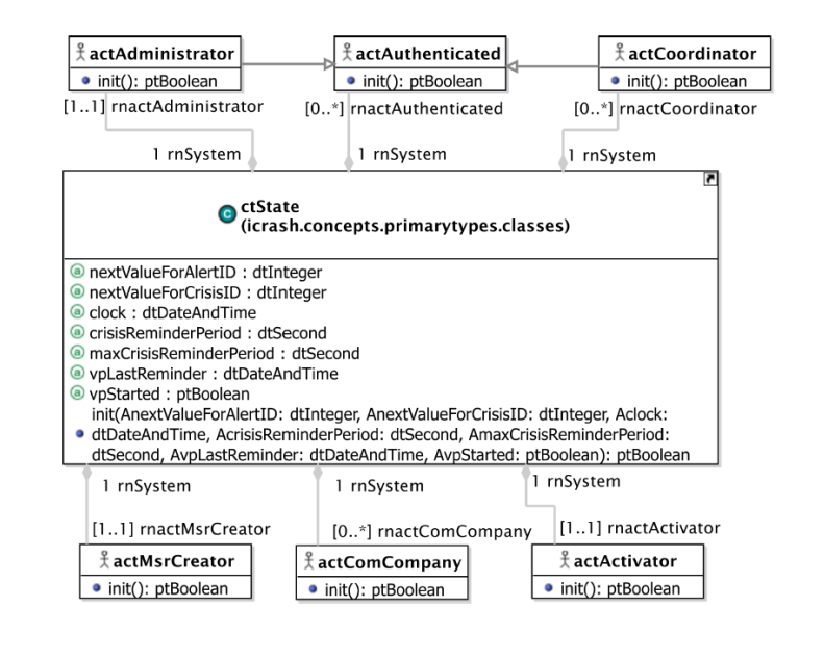
\includegraphics[width=0.9\textwidth]{./images/env_model.eps}
\end{center}
\caption{Environment Model}
\end{figure}

\newpage

% Technologies used to achieve the implementation
\chapter{Technological frameworks}
\label{chap:techFrm}


Here is provided a description of the technological frameworks used during the
development phase of the systemt. Such technological frameworks are properly
introduced and described from the point of view of their use during the
development of ths system. The iCrash application is supposed to be deployed
over at least 3 different computers: 1 database server, 1 application server,
and at least 1 client. 



\section{Eclipse}
\label{sec:Eclipse}
This IDE was required in order to interact with iCrash source files. It allowed
to check what is already written as well as to do additions. 


\section{Programming language}
\label{sec:Programming language}
Main programming language for this system is Java. It requires pre-installed SE
Development Kit (JDK) as well as the following DB systems: MySQL Server, MySQL
Workbench. 


\section{Vagrant}
\label{sec:Vagrant}
Distance launch of the system is possible due to the Vagrant, an open-source
software product for building and maintaining portable virtual development
environments. An suggested alternative is a Virtual Box.


\section{JavaFX}
\label{sec:JavaFX}
It is  is a software platform for creating and delivering desktop applications,
as well as rich internet applications (RIAs) that can run across a wide variety
of devices. It is used as a main GUI tool of the system.

\section{SceneBuilder}
\label{sec:SceneBuilder}
It is used as an IDE for GUI design and implementation with JavaFX









\newpage

% System architecture
\chapter{System Architecture}
\label{chap:arch}

This chapter presents information concerning the architecture of the software
system both from the static and dynamic viewpoints. The static viewpoint focuses
on the physical architecture (hardware) required to deploy and run the
software system along with the manner in which the components that make such
software system are grouped. On the other hand, the dynamic viewpoint focuses on
the behaviour of the software system at runtime. 

The static information is presented through the \gls{Deployment View} and the
\gls{Implementation View}. The dynamic aspects of the system are presented by
means of the \gls{UI Processing View}.


\section{Deployment view}
The aim of the \gls{Deployment View} is to describe the different processing nodes that compose
the deployment infrastructure and how they are interconnected. A processing node
corresponds to a piece of hardware aimed at executing either the whole software
system or a sub-part of it.




\section{Implementation view}
The \gls{Implementation View} describes each software system component and how
they are organised and combined to make the targeted software system.




\subsection{Component xx.yy.zz.c1}
TODO

\subsection{Component xx.yy.zz.c2}
TODO

\subsection{Component xx.yy.zz.c3}
TODO





\section{UI Processing view}
A \gls{UI Processing View} is aimed at explaining the required message exchanges
to achieve the launching of a system operation (specified in the \msrmessir
Analysis Document). These required message exchanges (which are not specified in
the \msrmessir Analysis Document) make part of the user interface (UI). Thus, the
main interest of a UI Processing View is to describe the design choices made
at the UI level, such that a system operation is launched. The description
of a UI Processing View is given by means of a UML Sequence Diagram. 


A complete Design Document should contain a UI Processing View for each
non-proactive system operation specified in the \msrmessir Analysis Document, as
such kind of system operations are launched by actors through UIs that allows
them to make so. 



\subsection{UI Processing view for system operation oeSystemOperation1}
TODO

 
\subsection{UI Processing view for system operation oeSystemOperation2}
TODO


\subsection{UI Processing view for system operation oeSystemOperation3}
TODO





\section{Non-functional runtime concerns}
The description of the runtime processes should be complemented with free
textual information regarding concurrency, distribution, performance and scalability aspects.


\subsection{Performance}
TODO



\subsection{Concurrency and Parallelism}
TODO




\subsection{Scalability}
TODO







\newpage

% Detailed Design
\chapter{Detailed design}
\label{chap:detDesign}


Provide an introduction to the proposed design. This introduction should help
the reader to understand the design choices made.


\section{Interaction Model}
An Interaction Model describes how each \gls{system operation} (that appears in the
Operation Model of the \msrmessir Requirements Analysis Model) is designed to meet
its specification. The design description of each system operation must be
focused on the messages exchanged between the different first-class objects
(i.e. instances of classes either included in Concept Model or introduced as
result of a design choice). An Interaction Model is modeled as a UML Sequence
Diagram.


\subsection{oeSetClock}
An active message used to statically set the date and time information in the
systems state.

\begin{figure}[H]
\begin{center}
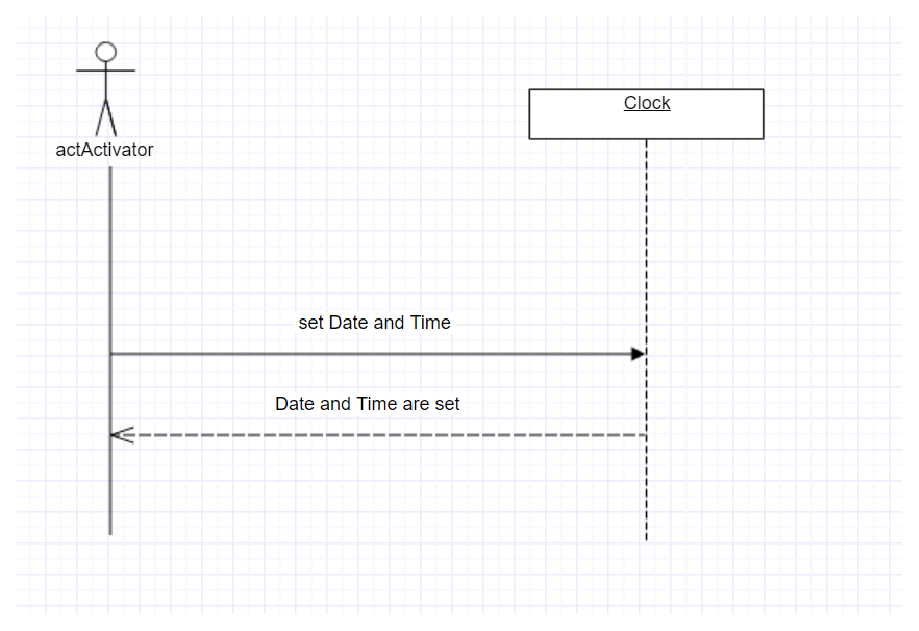
\includegraphics[width=0.5\textwidth]{./images/oeSetClock.eps} 
\end{center}
\caption{oeSetClock}
\end{figure}


\subsection{oeSollicitateCrisisHandling}
A proactive message (message of a pro-active actor with no parameter triggered
automatically if the pre protocol condition is true) used to avoid crisis to
stay too long in an not handled status
\begin{figure}[H]
\begin{center}
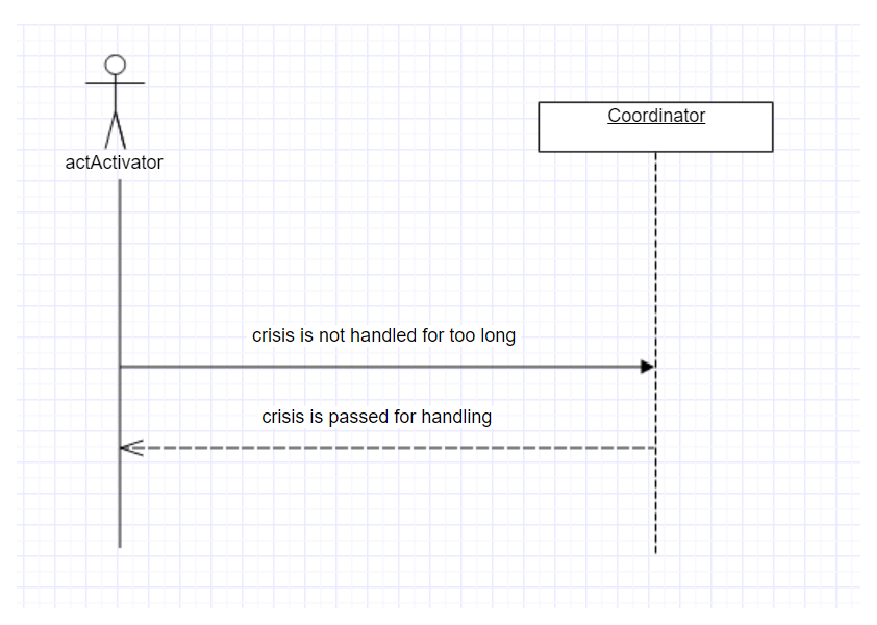
\includegraphics[width=0.5\textwidth]{./images/oeSollicitateCrisisHandling.eps} 
\end{center}
\caption{oeSollicitateCrisisHandling}
\end{figure}


\subsection{oeAddCoordinator}
Sent to add a new coordinator in the systems post state and environments post
state.
\begin{figure}[H]
\begin{center}
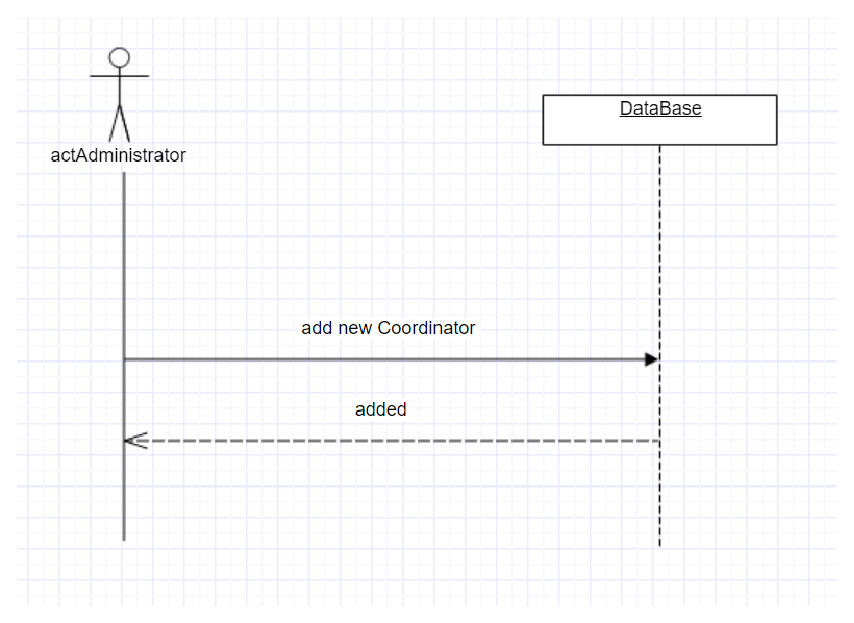
\includegraphics[width=0.5\textwidth]{./images/oeAddCoordinator.eps} 
\end{center}
\caption{oeAddCoordinator}
\end{figure}


\subsection{oeDeleteCoordinator}
Sent to delete an existing coordinator in the systems post state and
environments post state.
\begin{figure}[H]
\begin{center}
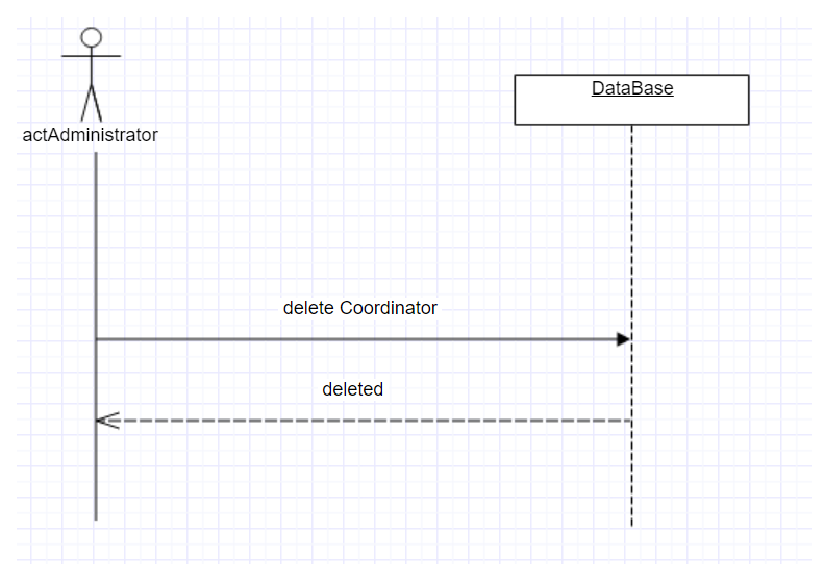
\includegraphics[width=0.5\textwidth]{./images/oeDeleteCoordinator.eps} 
\end{center}
\caption{oeDeleteCoordinator}
\end{figure}

\subsection{oeLogin}
Sent to request authorization to request access secured system operations.
\begin{figure}[H]
\begin{center}
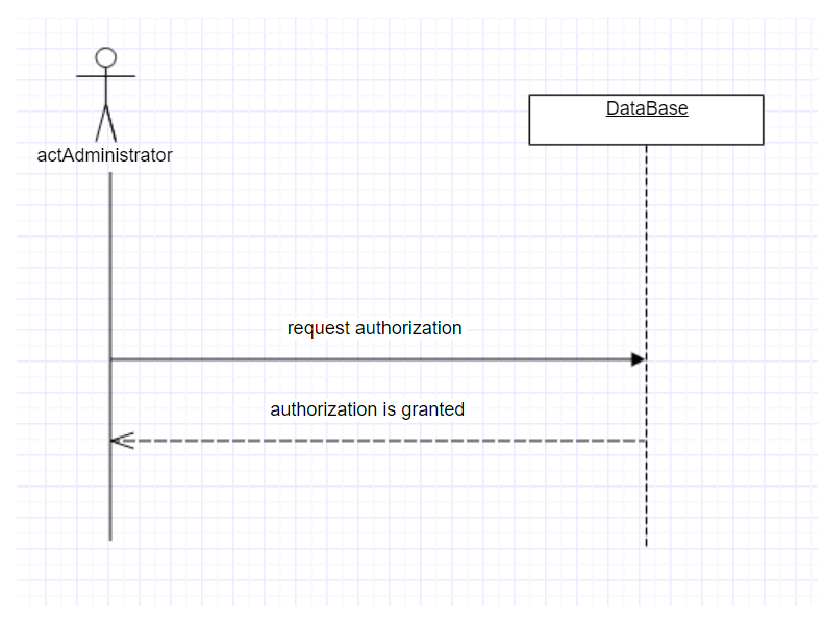
\includegraphics[width=0.5\textwidth]{./images/oeLogin.eps} 
\end{center}
\caption{oeLogin}
\end{figure}

\subsection{oeLogout}
Sent to end the secured access to specific system operations

\begin{figure}[H]
\begin{center}
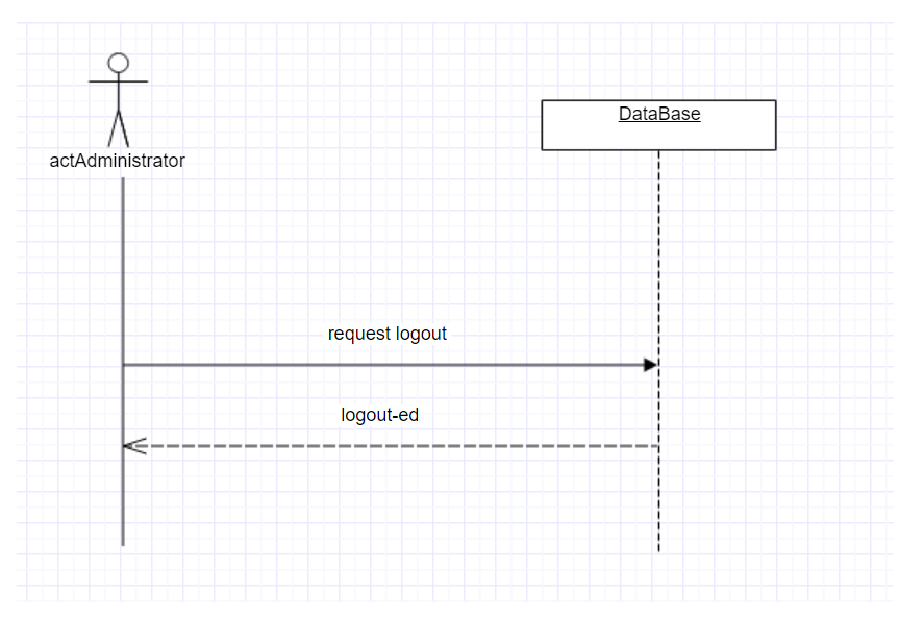
\includegraphics[width=0.5\textwidth]{./images/oeLogout.eps} 
\end{center}
\caption{oeLogout}
\end{figure}

\subsection{oeAlert}
Any human having a phone able to connect to the communication companies using
the iCrash system can send his company an sms message with structured
information in order to declare an alert

\begin{figure}[H]
\begin{center}
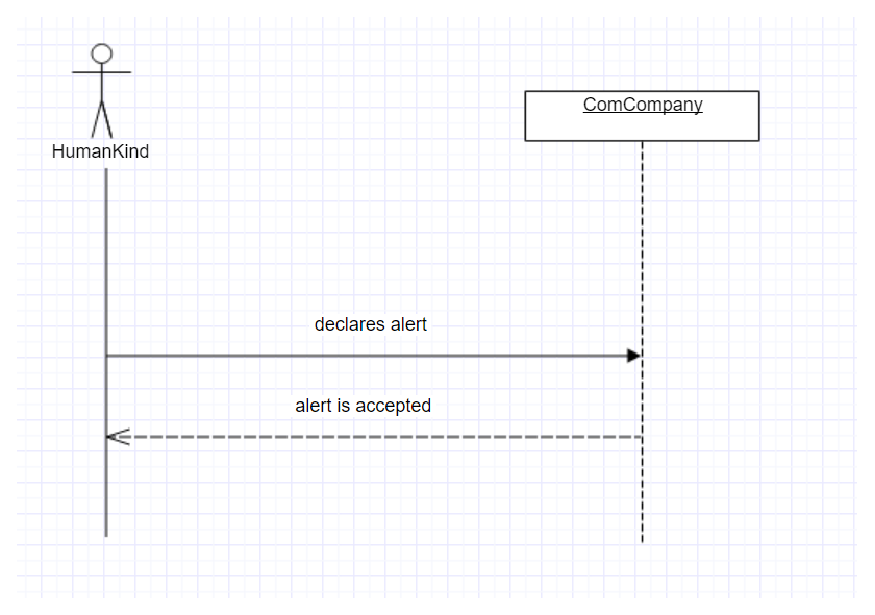
\includegraphics[width=0.5\textwidth]{./images/oeAlert.eps} 
\end{center}
\caption{oeAlert}
\end{figure}

\subsection{oeCloseCrisis}
Sent to indicate that a crisis should be considered as closed.

\begin{figure}[H]
\begin{center}
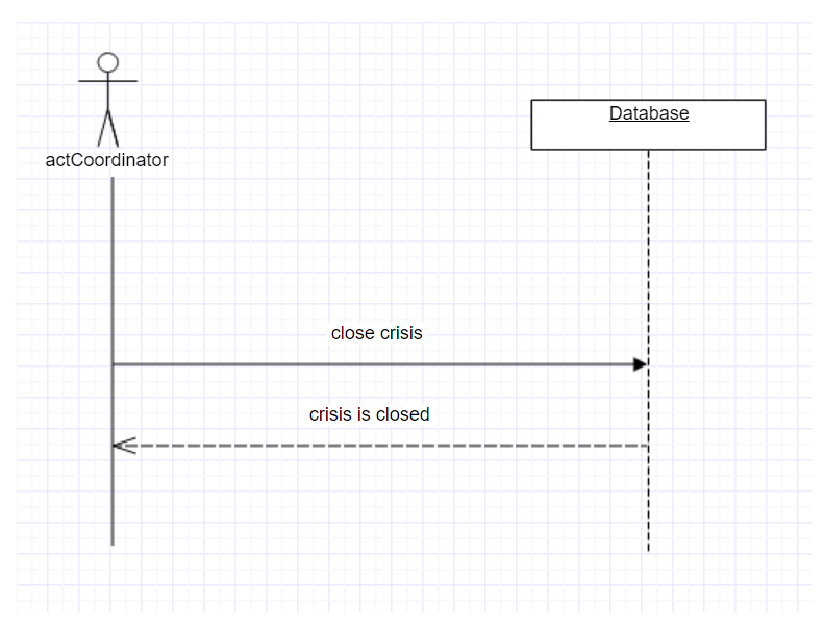
\includegraphics[width=0.5\textwidth]{./images/oeCloseCrisis.eps} 
\end{center}
\caption{oeCloseCrisis}
\end{figure}

\subsection{oeGetAlertsSet}
Sent to request all the ctAlert instances having a specific status.

\begin{figure}[H]
\begin{center}
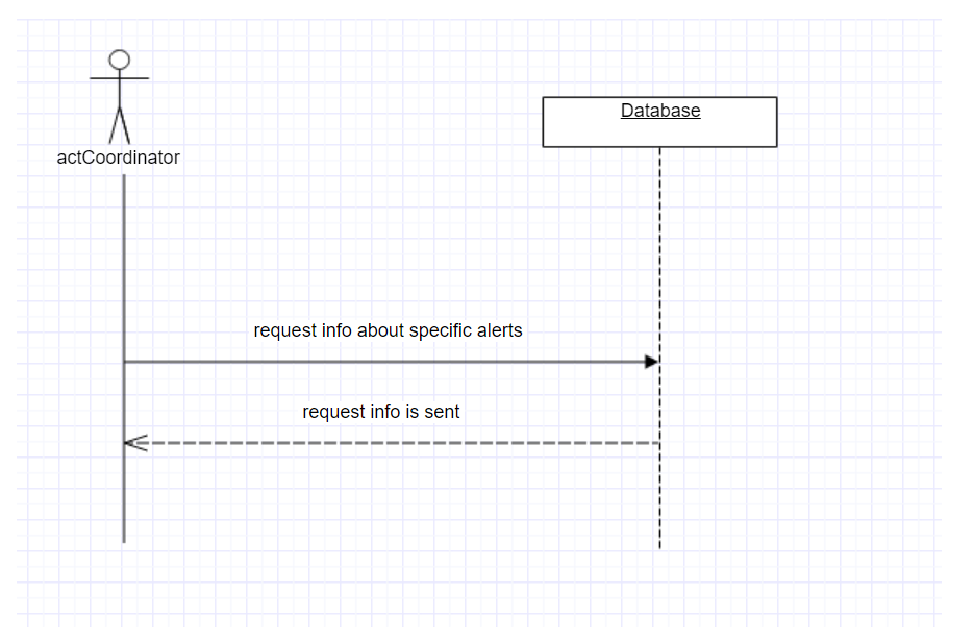
\includegraphics[width=0.5\textwidth]{./images/oeGetAlertsSet.eps} 
\end{center}
\caption{oeGetAlertsSet}
\end{figure}

\subsection{oeGetCrisisSet}
Sent to request all the ctCrisis instances having a specific status.

\begin{figure}[H]
\begin{center}
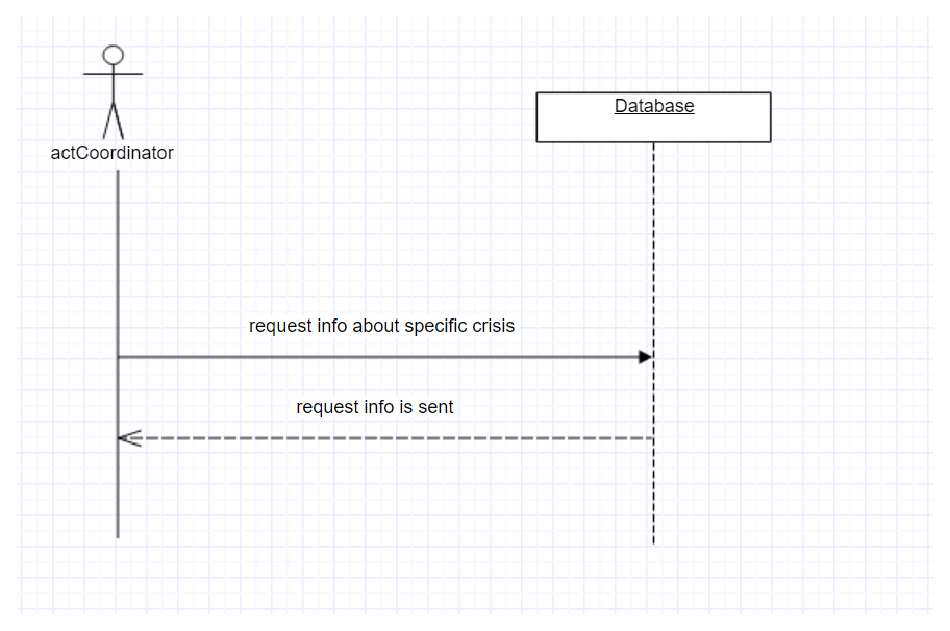
\includegraphics[width=0.5\textwidth]{./images/oeGetCrisisSet.eps} 
\end{center}
\caption{oeGetCrisisSet}
\end{figure}

\subsection{oeInvalidateAlert}
Sent to indicate that an alert should be considered as closed.

\begin{figure}[H]
\begin{center}
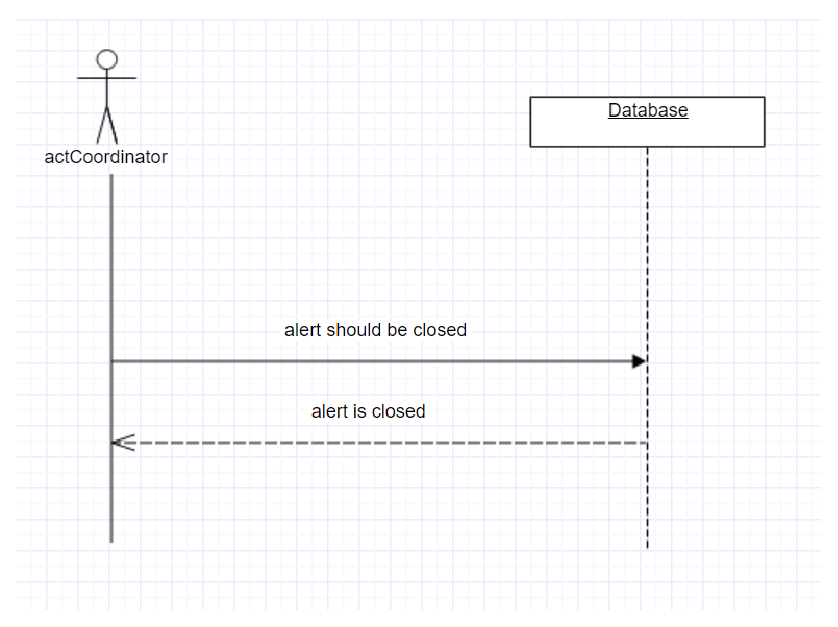
\includegraphics[width=0.5\textwidth]{./images/oeInvalidateAlert.eps} 
\end{center}
\caption{oeInvalidateAlert}
\end{figure}

\subsection{oeReportOnCrisis}
Sent to update the textual information available for a specific handled crisis.

\begin{figure}[H]
\begin{center}
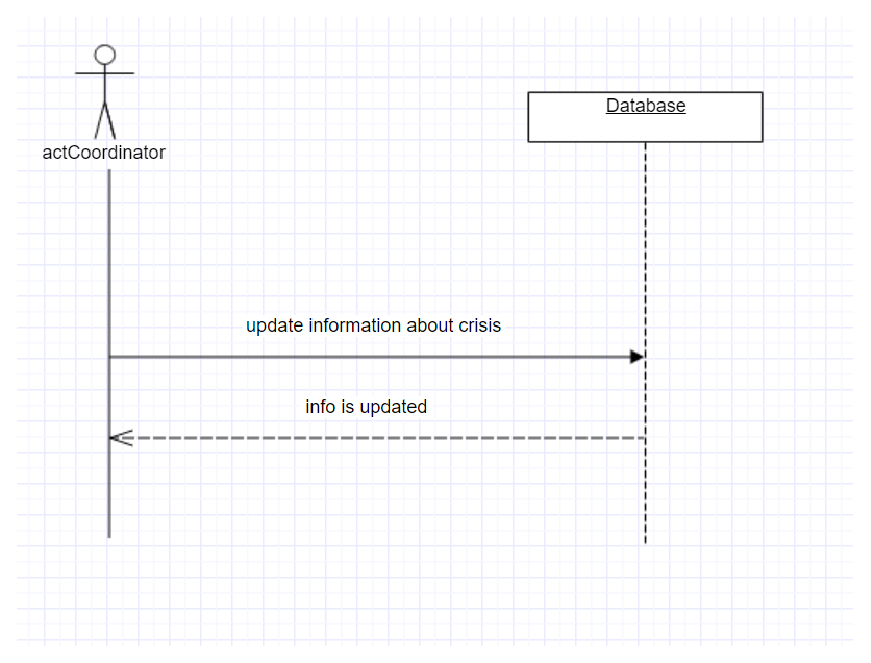
\includegraphics[width=0.5\textwidth]{./images/oeReportOnCrisis.eps} 
\end{center}
\caption{oeReportOnCrisis}
\end{figure}

\subsection{oeSetCrisisHandler}
Sent to declare himself as been the handler of a crisis having the specified id

\begin{figure}[H]
\begin{center}
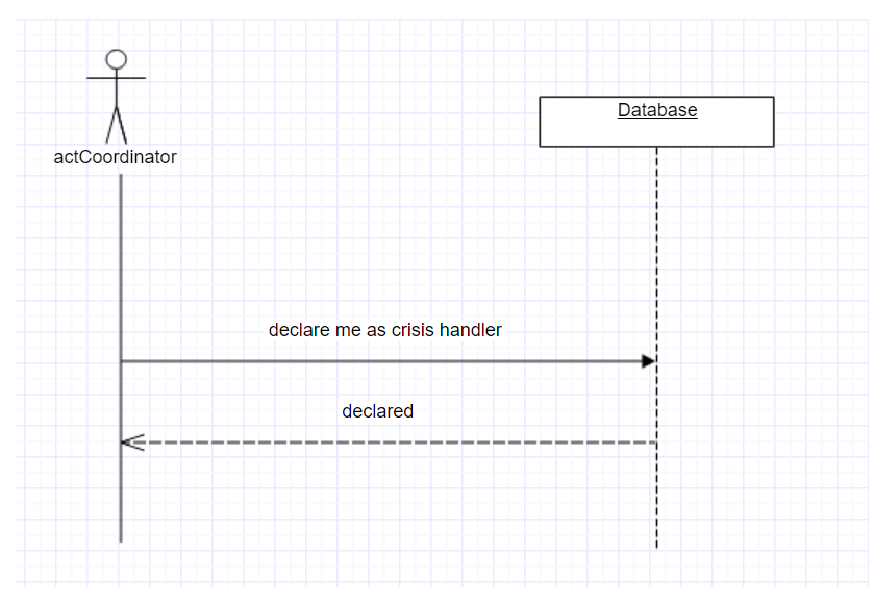
\includegraphics[width=0.5\textwidth]{./images/oeSetCrisisHandler.eps} 
\end{center}
\caption{oeSetCrisisHandler}
\end{figure}

\subsection{oeCreateSystemAndEnvironment}
oeCreateSystemAndEnvironment sent to request the initialization of the systems
class instances and the environment actors instances.

\begin{figure}[H]
\begin{center}
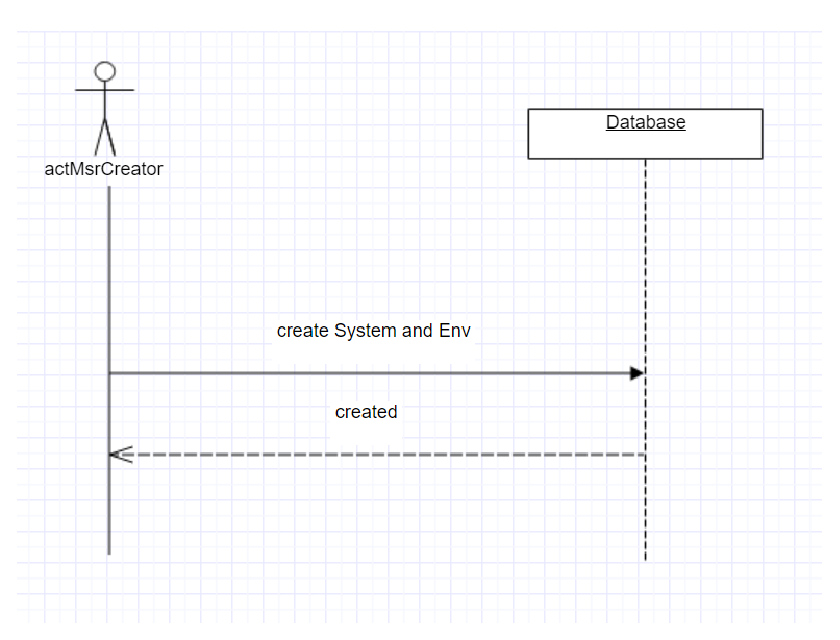
\includegraphics[width=0.5\textwidth]{./images/oeCreateSystemAndEnvironment.eps} 
\end{center}
\caption{oeCreateSystemAndEnvironment}
\end{figure}

\subsection{init}
init used to create an instance of the actor together with its interface
instances and update the assocations with the ctState instance.

\begin{figure}[H]
\begin{center}
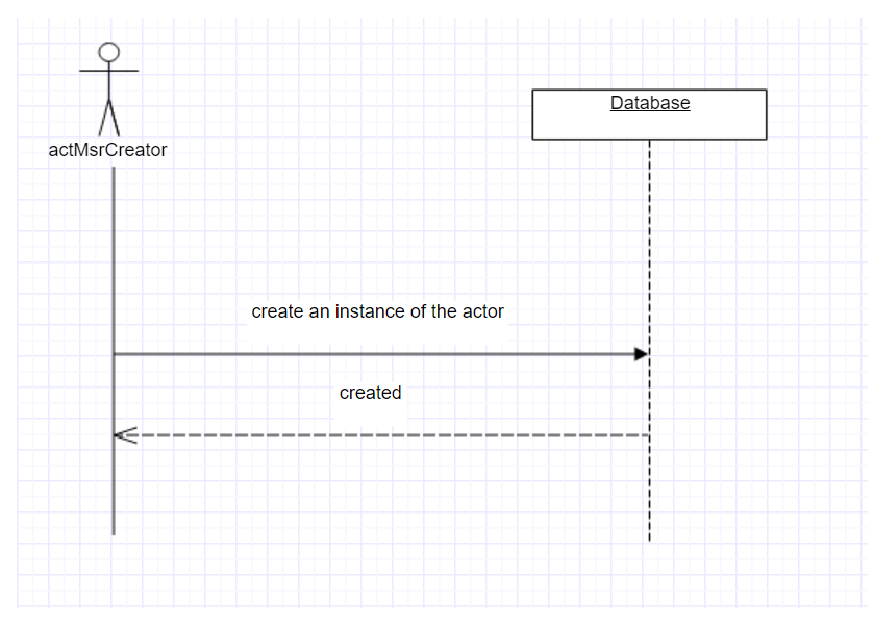
\includegraphics[width=0.5\textwidth]{./images/init.eps} 
\end{center}
\caption{init}
\end{figure}




\section{Design Class Model}
The Design Class Model is composed of the contents of all design classes (i.e.
every class appearing in at least one Interaction Model), all the navigable associations between design
classes, and the inheritance structure. The description of each class must
contain its attributes and operations. The Design Class Model is modeled as a
UML Class Diagram. 

It is advised to split the Design Class Model into multiple views as such model
may become pretty large. 
	

\subsection{Design Class Model view1}
TODO


\subsection{Design Class Model view2}
TODO



\subsection{Design Class Model view3}
TODO
\newpage

% Known limitations
\chapter{Known limitations}
\label{chap:know_limitations}


\section{General issues}
If you have any problems first try to visit
\url{http://messir.uni.lu:8090/confluence/questions/}. There you can post or
find some relevant information about your inquiry.


\section{Issue 1}
When administrator tries to log in through the admin system, it doesn't
accept that which is written in the readme file.\\

\noindent \textbf{Corrective actions}\\

1. The simplest way to know if all the VM are up and running is looking at the
messages that appear after you type vagrant up \\
2. Other thing you could try is to type in your console: vagrant box list .It
shows the different vagrant boxes already downloaded in your machine.\\
3. Also in case of using Vagrant project you need to check if all virtual
machines were started correctly. In particular you should login into the server
VM and see if the server has been started: you can do it by typing:  ps -ax |
grep java which displays all Java processes running on the machine.

\section{Issue 2}
At the moment system doesnot support mobile platforms such as iOS and Android.
In future we plane to extend supported platforms. However now it is mandatory to
use web version of the software.

\newpage


% Conclusion
\chapter{Conclusion}
\label{chap:final_conclusion}


TODO

\newpage

%APPENDICES
\appendix
% Last Modification:
% @author AUTHOR_NAME
% @date TODAY_DATE



\newpage

%GLOSSARY
%Uncomment the line below if you want to print all glossaries no matter if they
% appear in the document
%\glsaddall
\printglossaries
\newpage

%BIBLIOGRAPHY
\cleardoublepage
\bibliographystyle{./../lu.uni.lassy.excalibur.standard.report.libraries/styles/lncs} 
\bibliography{./../lu.uni.lassy.excalibur.standard.report.libraries/defs/references/messir,doc/bibliography/design}
\label{sec:references}
 
\end{document}
